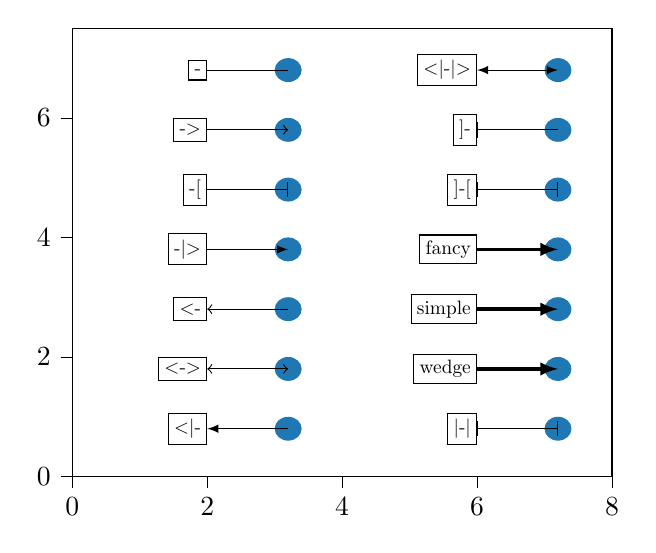
\begin{tikzpicture}

\definecolor{color0}{rgb}{0.12156862745098,0.466666666666667,0.705882352941177}

\begin{axis}[
tick align=outside,
tick pos=left,
x grid style={white!69.01960784313725!black},
xmin=0, xmax=8,
xtick style={color=black},
y grid style={white!69.01960784313725!black},
ymin=0, ymax=7.5,
ytick style={color=black}
]
\draw[fill=color0,draw opacity=0] (axis cs:3.2,6.8) circle (0.2);
\draw[fill=color0,draw opacity=0] (axis cs:3.2,5.8) circle (0.2);
\draw[fill=color0,draw opacity=0] (axis cs:3.2,4.8) circle (0.2);
\draw[fill=color0,draw opacity=0] (axis cs:3.2,3.8) circle (0.2);
\draw[fill=color0,draw opacity=0] (axis cs:3.2,2.8) circle (0.2);
\draw[fill=color0,draw opacity=0] (axis cs:3.2,1.8) circle (0.2);
\draw[fill=color0,draw opacity=0] (axis cs:3.2,0.8) circle (0.2);
\draw[fill=color0,draw opacity=0] (axis cs:7.2,6.8) circle (0.2);
\draw[fill=color0,draw opacity=0] (axis cs:7.2,5.8) circle (0.2);
\draw[fill=color0,draw opacity=0] (axis cs:7.2,4.8) circle (0.2);
\draw[fill=color0,draw opacity=0] (axis cs:7.2,3.8) circle (0.2);
\draw[fill=color0,draw opacity=0] (axis cs:7.2,2.8) circle (0.2);
\draw[fill=color0,draw opacity=0] (axis cs:7.2,1.8) circle (0.2);
\draw[fill=color0,draw opacity=0] (axis cs:7.2,0.8) circle (0.2);
\draw[-,black] (axis cs:2,6.8) -- (axis cs:3.2,6.8);
\node at (axis cs:2,6.8)[
  scale=0.7,
  fill=white,
  draw=black,
  line width=0.4pt,
  inner sep=3pt,
  anchor= east,
  text=black,
  rotate=0.0
]{-};
\draw[->,black] (axis cs:2,5.8) -- (axis cs:3.2,5.8);
\node at (axis cs:2,5.8)[
  scale=0.7,
  fill=white,
  draw=black,
  line width=0.4pt,
  inner sep=3pt,
  anchor= east,
  text=black,
  rotate=0.0
]{-$>$};
\draw[-|,black] (axis cs:2,4.8) -- (axis cs:3.2,4.8);
\node at (axis cs:2,4.8)[
  scale=0.7,
  fill=white,
  draw=black,
  line width=0.4pt,
  inner sep=3pt,
  anchor= east,
  text=black,
  rotate=0.0
]{-[};
\draw[-latex,black] (axis cs:2,3.8) -- (axis cs:3.2,3.8);
\node at (axis cs:2,3.8)[
  scale=0.7,
  fill=white,
  draw=black,
  line width=0.4pt,
  inner sep=3pt,
  anchor= east,
  text=black,
  rotate=0.0
]{-$|$$>$};
\draw[<-,black] (axis cs:2,2.8) -- (axis cs:3.2,2.8);
\node at (axis cs:2,2.8)[
  scale=0.7,
  fill=white,
  draw=black,
  line width=0.4pt,
  inner sep=3pt,
  anchor= east,
  text=black,
  rotate=0.0
]{$<$-};
\draw[<->,black] (axis cs:2,1.8) -- (axis cs:3.2,1.8);
\node at (axis cs:2,1.8)[
  scale=0.7,
  fill=white,
  draw=black,
  line width=0.4pt,
  inner sep=3pt,
  anchor= east,
  text=black,
  rotate=0.0
]{$<$-$>$};
\draw[latex-,black] (axis cs:2,0.8) -- (axis cs:3.2,0.8);
\node at (axis cs:2,0.8)[
  scale=0.7,
  fill=white,
  draw=black,
  line width=0.4pt,
  inner sep=3pt,
  anchor= east,
  text=black,
  rotate=0.0
]{$<$$|$-};
\draw[latex-latex,black] (axis cs:6,6.8) -- (axis cs:7.2,6.8);
\node at (axis cs:6,6.8)[
  scale=0.7,
  fill=white,
  draw=black,
  line width=0.4pt,
  inner sep=3pt,
  anchor= east,
  text=black,
  rotate=0.0
]{$<$$|$-$|$$>$};
\draw[|-,black] (axis cs:6,5.8) -- (axis cs:7.2,5.8);
\node at (axis cs:6,5.8)[
  scale=0.7,
  fill=white,
  draw=black,
  line width=0.4pt,
  inner sep=3pt,
  anchor= east,
  text=black,
  rotate=0.0
]{]-};
\draw[|-|,black] (axis cs:6,4.8) -- (axis cs:7.2,4.8);
\node at (axis cs:6,4.8)[
  scale=0.7,
  fill=white,
  draw=black,
  line width=0.4pt,
  inner sep=3pt,
  anchor= east,
  text=black,
  rotate=0.0
]{]-[};
\draw[-latex,very thick,black] (axis cs:6,3.8) -- (axis cs:7.2,3.8);
\node at (axis cs:6,3.8)[
  scale=0.7,
  fill=white,
  draw=black,
  line width=0.4pt,
  inner sep=3pt,
  anchor= east,
  text=black,
  rotate=0.0
]{fancy};
\draw[-latex,very thick,black] (axis cs:6,2.8) -- (axis cs:7.2,2.8);
\node at (axis cs:6,2.8)[
  scale=0.7,
  fill=white,
  draw=black,
  line width=0.4pt,
  inner sep=3pt,
  anchor= east,
  text=black,
  rotate=0.0
]{simple};
\draw[-latex,very thick,black] (axis cs:6,1.8) -- (axis cs:7.2,1.8);
\node at (axis cs:6,1.8)[
  scale=0.7,
  fill=white,
  draw=black,
  line width=0.4pt,
  inner sep=3pt,
  anchor= east,
  text=black,
  rotate=0.0
]{wedge};
\draw[|-|,black] (axis cs:6,0.8) -- (axis cs:7.2,0.8);
\node at (axis cs:6,0.8)[
  scale=0.7,
  fill=white,
  draw=black,
  line width=0.4pt,
  inner sep=3pt,
  anchor= east,
  text=black,
  rotate=0.0
]{$|$-$|$};
\end{axis}

\end{tikzpicture}
